\scanpage{51}
\mspage{13}
\[
\mathcal H^0:\widetilde C_A\longrightarrow\widehat C_A \qquad(10)
\]
le foncteur d'injection des faisceaux dans les préfaisceaux.
Le foncteur $\mathcal H^0$ est un foncteur exact à gauche (2.3.14.II).
Ses foncteurs dérivés \unsure{droitsseront|droits seront} notés :
\[
\mathcal H^q:\widetilde C_A\longrightarrow\widehat C_A \qquad(11)
\]
Pour tout objet $X$ de $C$ \deleted{,\unsure{on a}} et pour tout A-Module $F$, on a :
\[
\inserted{\mathcal H^q(F)(X)}\;\deleted{\unsure{t|\dagger}\,\unsure{\mathcal H^q|H^q}}\;
\deleted{H^0(\unsure{\widehat C}/X,\mathcal H^q(F))}=H^q(\widetilde C/X,F)\qquad(12)
\]
En effet pour $q=0$, cet isomorphisme résulte immédiatement des définitions. On l'en déduit pour tout $q$ en remarquant que le foncteur ``section\inserted{s} sur $X$'' est exact \deleted{\unsure{à|d}} sur la catégorie des préfaiscea\deleted{\illegible{2}}\unsure{ux}.

Soit $L:\widehat C\longrightarrow\widehat C$ le foncteur défini en (2.3.11.II).
Le foncteur $L$ commute aux limites projectives finies et par suite transforme \margin{\raisebox{.7ex}{$\unsure{\rho}$}\,\inserted{les}} $\unsure{\rho}$ préfaisceaux d' A-modules en préfaisceaux de A-modules. Nous noterons :
\[
\check{\mathcal H}^{0}:\widehat C_A\longrightarrow\widehat C_A \qquad(13)
\]
\margin{\figure{\begin{tikzpicture}[x=1mm,y=1mm]
\draw[line width=0.3pt,black!30] (0,46.9) -- (9,46.5);
\draw[line width=0.25pt,black!20] (9,46.5) -- (9,0.2);
\draw[line width=0.3pt,black!45] (9,44.8) -- (9,43.2) (9,42.7) -- (9,41.9);
\draw[line width=0.5pt,black!75] (0,0.6) .. controls (3,0.25) and (6,0.05) .. (9,0.2);
\end{tikzpicture}}}
\margin{\figure{\begin{tikzpicture}[x=1mm,y=1mm]
\draw[line width=0.5pt,black!40] (0,0) -- (1.8,2.2);
\draw[line width=0.7pt] (1.3,1.6) -- (1.8,2.2);
\end{tikzpicture}}}
le foncteur induit par $L$ sur les préfaisceaux de A-modules.
Le foncteur $\check{\mathcal H}^0$ est exact à \deleted{droite} gauche. Ses foncteurs dérivés droits seront notés $\check{\mathcal H}^q$. \deleted{Les préfai} Soit $G$ un préfaisceau de A-modules. Les préfaisceaux $\check{\mathcal H}^q(G)$ seront appelés les préfaisceaux de \begingroup
\setbox0=\hbox{cohomologie de \v{C}ech du}
\dimen0=\wd0 \advance\dimen0 by 8pt
\dimen2=\ht0 \advance\dimen2 by \dp0 \advance\dimen2 by 8pt
\leavevmode\rlap{\raisebox{\dimexpr-\dp0-4pt\relax}{%
\begin{tikzpicture}[x={\dimexpr\dimen0/390\relax},y={\dimexpr-\dimen2/80\relax},line width=.3pt]
\path[use as bounding box] (0,0) rectangle (390,80);
\draw (22,65) .. controls (130,66) and (261,68) .. (365,69);
\end{tikzpicture}}}%
\kern4pt\box0\kern4pt\endgroup préfaisceau $G$.

Ppour tout objet $X$ de $C$, on a un isomorphisme canonique :
\begingroup
\setbox0=\hbox{%
  \let\ScanOverlaySavedSout\sout
  \let\sout\relax
  \deleted{%
    \let\sout\ScanOverlaySavedSout
    \parbox{.95\linewidth}{\[\deleted{\unsure{H^0(\widehat C, H^0(\widehat C/X,\qquad(G)))=\operatorname{Lim}}}\]\[H^0(\widehat C/X,\qquad(G))=\underset R{\operatorname{Lim}}\,H^q(\widehat C/R,G)^{C}\]En effet pour $q=0$, cet isomorphisme résulte immédiatement\\des définitions}}}
\dimen0=\wd0 \advance\dimen0 by 8pt
\dimen2=\ht0 \advance\dimen2 by \dp0 \advance\dimen2 by 8pt
\leavevmode\rlap{\raisebox{\dimexpr-\dp0-4pt\relax}{%
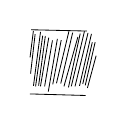
\begin{tikzpicture}[x={\dimexpr\dimen0/1045\relax},y={\dimexpr-\dimen2/265\relax},line width=.3pt]
\path[use as bounding box] (0,0) rectangle (1045,265);
\draw (51,8) -- (900,13);
\draw (35,255) -- (880,261);
\draw (36,114) -- (87,12);
\draw (44,177) -- (113,25);
\draw (88,224) -- (195,16);
\draw (120,226) -- (228,31);
\draw (166,223) -- (268,32);
\draw (194,226) -- (320,38);
\draw (257,226) -- (376,49);
\draw (313,246) -- (451,43);
\draw (381,218) -- (509,48);
\draw (437,214) -- (626,14);
\draw (502,215) -- (683,19);
\draw (551,226) -- (762,36);
\draw (619,230) -- (797,23);
\draw (662,226) -- (862,14);
\draw (719,226) -- (916,20);
\draw (787,224) -- (968,24);
\draw (836,217) -- (981,56);
\draw (874,222) -- (1024,56);
\draw (907,232) -- (1039,108);
\end{tikzpicture}}}%
\kern4pt\box0\kern4pt\endgroup
\[
\inserted{\check{\mathcal H}^q(G)(X)}\;\deleted{H^0(\unsure{\widehat C}/X,\check{\mathcal H}^q(G))}
=\vcenter{\hbox{\begingroup
\setbox0=\hbox{$\displaystyle \underset{R}{\underset{\longrightarrow}{\operatorname{Lim}}}$}
\dimen0=\wd0 \advance\dimen0 by 18pt
\dimen2=\ht0 \advance\dimen2 by \dp0 \advance\dimen2 by 16pt
\rlap{\raisebox{\dimexpr-\dp0-8pt\relax}{%
\begin{tikzpicture}[x={\dimexpr\dimen0/64\relax},y={\dimexpr-\dimen2/70\relax},line width=.3pt]
\path[use as bounding box] (0,0) rectangle (64,70);
\draw (2,31)--(14,3);
\end{tikzpicture}}}%
\kern9pt\box0\kern9pt\endgroup}}\,H^q(\widehat C/R,G)\qquad(14)
\]
\shortstack[l]{\inserted{Comme}\\\deleted{Ainsi qu'}} il resulte immédiatement des définitions (2.3.11.II).

(Dans cette formule la limite inductive est prise suivant la catégorie des cribles couvrants $X$).
\margin{50}

